\documentclass[12pt]{article}
\usepackage{amsmath}
\usepackage{amsthm}
\usepackage{amssymb}
\usepackage{enumerate}
\usepackage{graphicx}
%\usepackage{fullpage}
\usepackage[top=1in, bottom=1in, left=0.8in, right=1in]{geometry}
\usepackage{multicol}
\usepackage{wrapfig}
\usepackage{units}
\usepackage{setspace}
\doublespacing

\setlength{\columnsep}{0.1pc}

\title{Ropes - Alternative String Representation}
\author{Leo Martel, Paul Martinez, Andy Moreland}
\date{\today}
\begin{document}

\maketitle
\vspace{-0.3in}
\rule{\linewidth}{0.4pt}

%%%%%%%%%%%%%%%%%%%%%%%%%%%%%%%%%%%%%%%%%%%

\section{Introduction}

In this paper we will discuss the Rope data structure, a data structure intended to serve as a more robust and more performant alternative to the traditional String type offered in most languages.
The seminal paper regarding Ropes was written by Hans-J. Boehm, Russ Atkinson and Michael Plass in 1995.
We will provide an overview of their paper, beginning with their justification for Ropes in the first place.
We will continue with a more technical exploration of the implementation details and running time guarantees of the various operations that Ropes support.
Finally, we will conclude with an overview of our contributions. In particular, we have implemented our own Rope in $C++$ and we provide benchmarks that demonstrate its performance. We have also implemented a $D3$\footnote{http://d3js.org/} based visualization which helps demonstrate the internal workings of a rope. We briefly discuss this implementation before we conclude.

\section{Justification for Expanded String Type}

Historically languages like C and Pascal have implemented strings essentially as arrays of characters. Generally this array is of fixed length and basic operations can be implemented in terms of standard array access. Higher level operations are usually provided in the form of library functions: C, for example, provides substring, concatenation and length operations. Many languages implement the string type in the most bare-bones way possible: C, for example, does not even include length alongside the character data.

Boehm, Russ and Plass (BRP) begin their paper by discussing the problems that follow from this type of approach. They suggest the Rope datastructure and demonstrate that it improves on many of these flaws. We will summarize their ideas here.

BRP believe that one of the biggest problems with traditional arrays is the fact that they are mutable. Robust system design dictates that we separate our systems into a collection of modules which interact over tightly-guarded interfaces. Unfortunately, for the sake of efficiency strings are often passed through these interfaces by reference. This means that the client of a given module must take care not to accidentally modify a string that it receives lest it incidentally change the internal state of the module. This violates the Principle of Encapsulation. Accordingly, BRP have designed the Rope data structure to efficiently support important operations while remaining immutable: the Rope is a copy-on-write structure.

In additional to enabling immutability, BRP's Rope design supports efficient concatenation, substring and deletion operations which do not require excessive space overhead. At the time of writing this was particularly relevant because, as BRP joke, "six-month-old child randomly typing at a workstation would routinely crash some older UNIX kernels due to a buffer size limitation." Even editors which are now considered efficient, like vi, used to struggle with long line lengths. By contrast, the Rope structure scales well to handle large strings.

\section{Implementation and Running Time}

In this section we will discuss the representation of the Rope datastructure as well as the implementaton and running times of various common operations on it.

First, we will develop the representation. As a motivating example, consider the concatenation of two strings. If we want to support immutability naively we might decide to copy both strings into a new buffer. However, this is extremely performance inefficient if the strings are large, and requires making full duplicates of the strings before we have actually modified anything. This suggests that a reasonable approach would be to try to loosely join our target strings together: in particular, we will gradually form a tree structure of joined strings.

More directly: a Rope is a binary tree whose interior nodes are called \emph{concatenation nodes}, since they represent the concatenation of two smaller strings, and whose leaves are \emph{flat} strings which are represented as character arrays. BRP note that because the leaf notes are immutable, a sequence of concatenation and substring calls could lead to many of these nodes being shared among multiple ropes. Technically this would make the Rope a directed acyclic graph rather than a tree, but for the sake of brevity we will refer to the structure as a tree since we will generally be considering only a single rope at a time.

By virtue of this tree structure, alongside a few minor adjustments, our Rope structure is able to efficiently support the following operations, where $n$ is taken to be the length of the string represented by the Rope:

\begin{enumerate}
\item \emph{charAt(i)}: returns the character stored at index $i$ in time $O(\log(n))$
\item \emph{concat$(r_1, r_2)$}: returns a new rope structure which contains $r_1$ followed by $r_2$ in time $O(1)$
\item \emph{substring(i, j)}: returns a new rope structure consisting of the characters between (inclusive) indices $i$ and $j$ in time $O(\log(n)$
\item \emph{iteration} over each character more efficiently than by repeated charAt calls in time $O(n)$
\end{enumerate}

These running times all assume a balanced-tree representation. However, BRP argue in the paper that tree-rebalancing operations are very expensive in practice and so should be avoided when possible. In practice, this may cause some of these asymptotic bounds to slip. 

In the following subsections we will describe how each of these operations is implemented.

\subsection{Concatenation}

A common use case for strings is continaully concatenation at one end. Thus whenever the right argument is a string literal, we would like to avoid growing the tree excessively. We can do this by accounting for two cases. One, if both arguments are string literals, we will simply combine them into a new string literal. Two, if the left argument is a concatenation node but its right child is a string literal, then we will combine the right child with the right argument to form a new string literal and then return a new concatenation node with the left child. In other cases we simply create a new concatenation node. These two rules make the case of continually appending to the end of a string very efficient.

\subsection{Substring}

When taking substrings

\section{Benchmarking}

We wrote some code.

\section{Visualization}

In order to better visualize how a rope structure may be built up, we set out to write a simple text editor whose backing store is a Rope. Text editors are one of the more commonly cited uses for Ropes, so it seemed fitting. Accompanying the editor is a tree structure displaying the current state of the rope's internal representation.

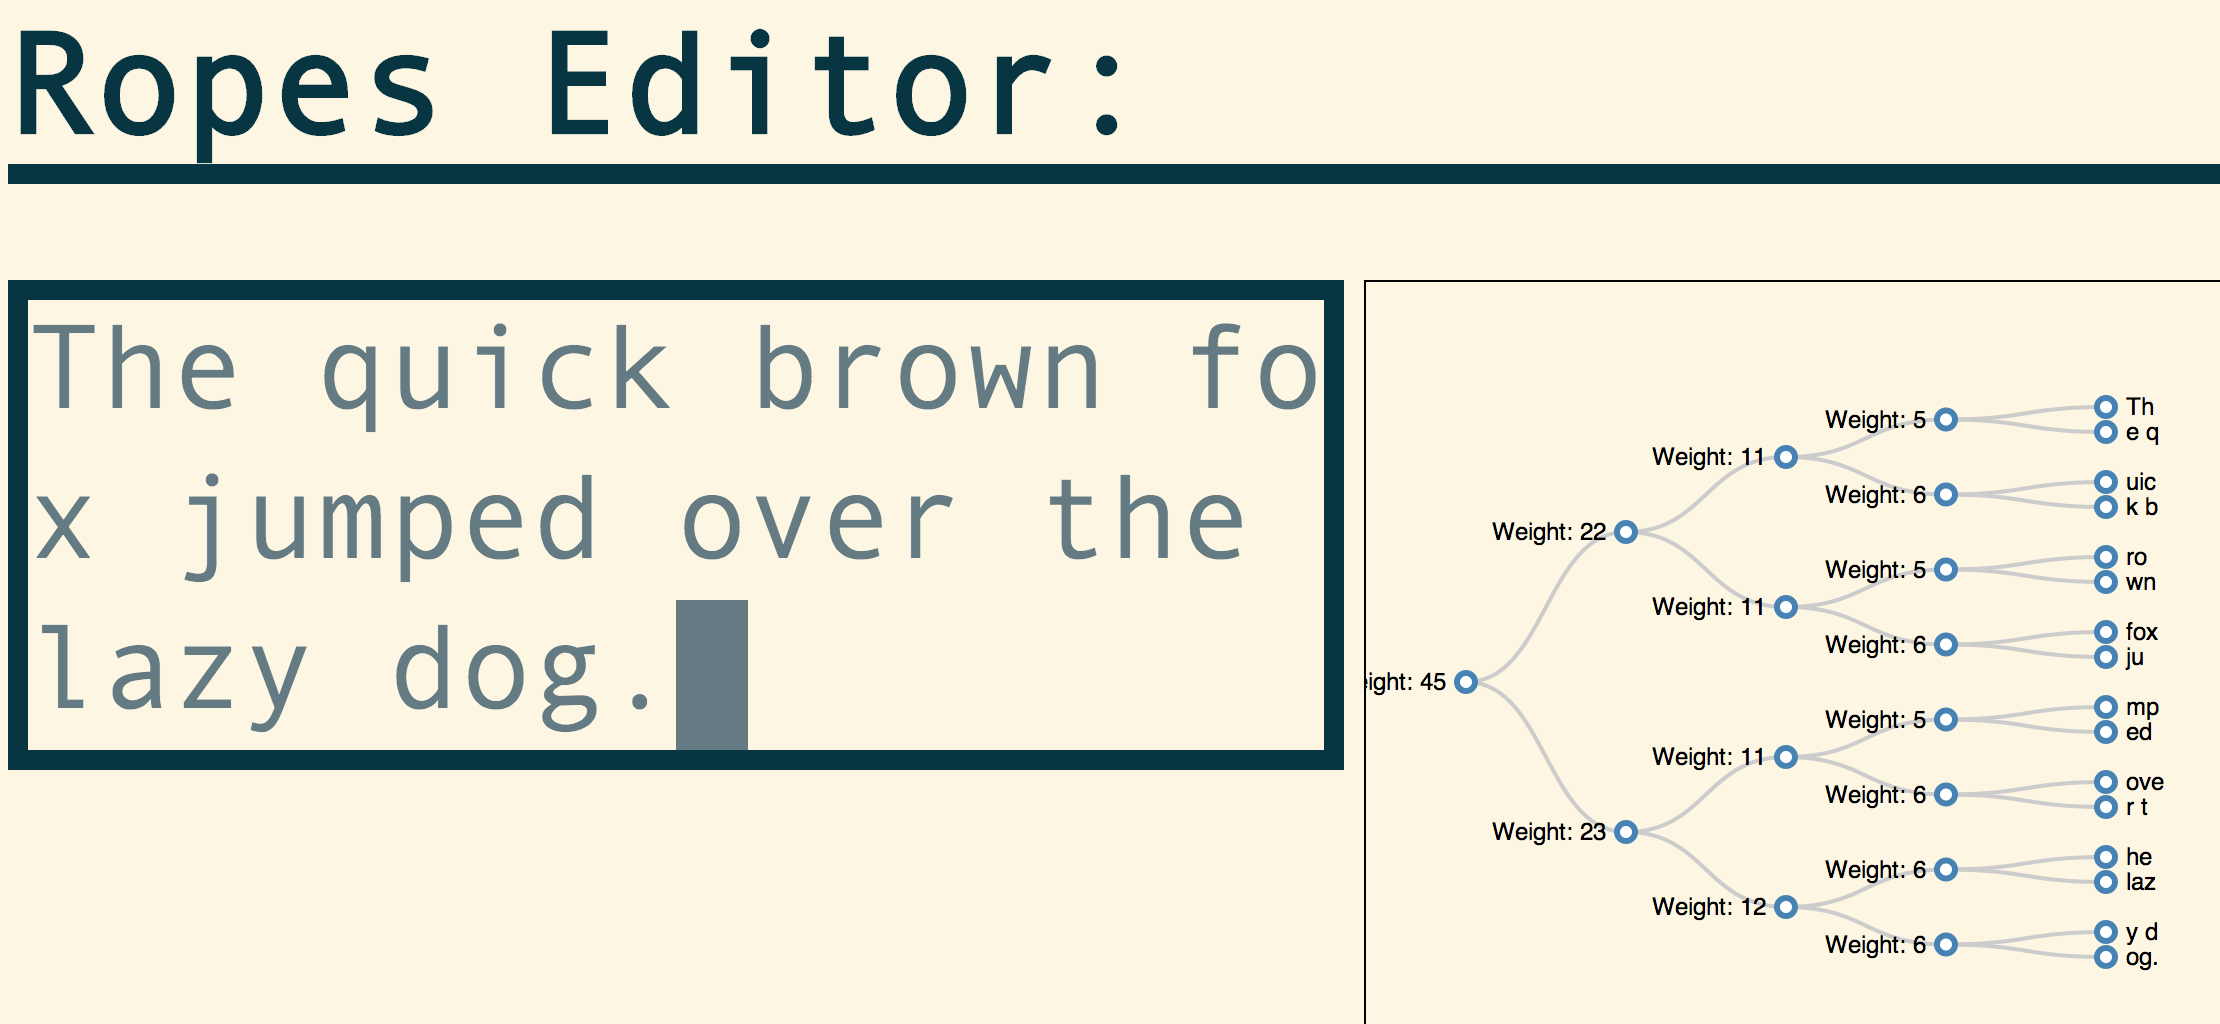
\includegraphics[scale=0.25]{editorImage1}

In building this simple demo, we began to consider some of the limitations of Ropes. While the immutability requirement may grant certain safety benefits, one could argue that it in a sense causes more trouble than it is worth. Consider a case where a large file has been build up via a series of sequential inserts at the end of the string. Then, when a character in the middle of the string is deleted. In the traditional implementation this first delete would require new concatenation nodes to be constructed all the way along the path from the root of the tree to node containing the edited string. Each subsequent insertion or deletion would continue to create a lot of work, including potentially memory allocations. In a text editor one often does a lot of local edits. It would be nice if a so-called `working-set' were located near the root of the tree. (We will ignore the fact that the bottleneck in most text editors these days is not the actual text manipulation but the neurons of the typist. We can still continue the exercise.)

One could use a splay tree for the this purpose, but then one completely forfeits some of the subtler niceties afforded by the immutability principle. For example, one could easily implmement an undo stack (very useful in a text editor!) by simply maintaining a list to previous representations of the file's string. Out of curiosity, we will forget this feature and continue to see what alterations we can apply. Suppose that in addition to having a completely mutable tree, we also had mutable string buffers. Then a series of local edits would splay a node up to the root, and as long as the buffer was moderately full every insert/delete would only take time proportional to the size of the buffer. This unfortunate fact means that this approach is unlikely to lead to any asymptotically better algorithms. We can see this by assuming that we have a block size of $b$. Though this hasn't been mentioned, supose we could somehow force each buffer to be at least half full. This would guarantee $\Theta(n/b)$ nodes in our tree, so splaying would take $O(\log n/b)$, but every individual operation at a node would also take $O(b)$ for a total time of $O(\log n/b) + O(b) = O(\log n) - O(\log b) + O(b) = O(\log n) + O(\log )$, which is nothing special. As long as $b$ on the order of $\log n$, then we won't lose any ground. Perhaps such a structure would be faster in practice due to the fewer allocations. As mentioned, insertions and deletions from the middle could force $O(\log n)$ new nodes per operation in the immutable rope, where as in this its $O(1 / \log n)$ allocations per insertion or deletion because you only would need a new node wheneve you add $\log n$ new characters! This is certainly better and likely indicates significant performace benefits.


\end{document}
